\documentclass[a4paper,french,10pt]{article}
\usepackage{homework}
\usepackage{diagbox}

% change le nom de la table des matières
\addto\captionsfrench{\renewcommand*\contentsname{Sommaire}}

\lstdefinelanguage{R}%
{morekeywords={function,for,in,if,elseif,else,TRUE,FALSE,%
		return, while, diag, sum, sqrt, nrow, ncol, par, plot, cbind, rep, as, survdiff, survreg, ifelse, anova,
		row, names, colnames, mean, data, frame, model, in, list, rexp, rpois, summary,
		matrix, TRUE, FALSE, for, if, else, function, NA, print, survfit, Surv, rho, ggplot},%
	sensitive=true,%
	morecomment=[l]{\#},%
	morestring=[s]{"}{"},%
	morestring=[s]{'}{'},%
}[keywords,comments,strings]%

\lstset{%
	language         = R,
	basicstyle       = \ttfamily,
	keywordstyle     = \bfseries\color{blue},
	stringstyle      = \color{magenta},
	commentstyle     = \color{olive},
	showstringspaces = false,
}

\begin{document}
	
	% Blank out the traditional title page
	\title{\vspace{-1in}} % no title name
	\author{} % no author name
	\date{} % no date listed
	\maketitle % makes this a title page
	
	% Use custom title macro instead
	\usebox{\myReportTitle}
	\vspace{1in} % spacing below title header
	
	% Assignment title
	{\centering \huge \assignmentName \par}
	{\centering \noindent\rule{4in}{0.1pt} \par}
	\vspace{0.05in}
	{\centering \courseCode~: \courseName~ \par}
	{\centering Rédigé le \pubDate\ en \LaTeX \par}
	\vspace{1in}
	
	% Table of Contents
	\tableofcontents
	\newpage
	
	%----------------------------------------------------------------------------------------
	%	EXERCICE 1
	%----------------------------------------------------------------------------------------
	

\section{Introduction}
Dans le cadre de ce projet, nous allons modéliser le comportement extrême des vagues dans le golfe du lion à l'aide des méthodes vue à travers l'unité d'enseignement HAX005X "valeurs extrêmes". D'après la source \cite{golfLion}, le golf s'étale sur 220 kilomètres de la Camargue à la frontière espagnole. La côte, essentiellement sableuse, a été façonnée par la houle (la mer gagnant souvent les terres par élévation du niveau marin) et l'érosion côtière. L'apport de sédiments en provenance des fleuves a également permis de faire avancer le rivage pendant de longues périodes. Des formations de lagunes "comme les graus" (parfois temporaires) ont pu apparaitre et ont permis de faire communiquer les étangs littoraux avec la mer. Le golf du Lion est donc un milieu naturellement dynamique. C'est dans ce contexte que nous étudions le comportement extrême des vagues à cet endroit, de façon univariée dans un premier temps puis de façon bivariée dans un second temps. 

\newpage

\section{Présentation des données}

Les données que nous avons à notre disposition pour ce projet sont les suivantes:
\begin{itemize}
	\item \textbf{DonneesStations}
	\item \textbf{DonneesVagues}
\end{itemize}
Pour réaliser les analyses, nous utiliserons essentiellement les données en provenance du dataframe \textit{DonneesVagues} qui correspondent à des enregistrements de hauteurs de vagues significatives horaires de 20 stations situées dans le golf du Lion. Ces mesures horaires ont été enregistrées de 1961 à 2012. Ce dataframe est constitué de 464280 observations (en lignes) et de 21 variables (en colonnes). Décrivons un peu plus en détail les colonnes de ce dataframe \textit{DonneesVagues}:
\begin{itemize}
	\item \textbf{date} nous renseigne sur la date (format année mois jours) et l'heure précise (format heure minute seconde) à laquelle a été enregistrée la mesure.
	\item \textbf{station 1 à 20} nous renseigne sur les hauteurs de vagues mesurées
\end{itemize}
Le deuxième dataframe \textit{DonneesStations}, quant à lui nous renseigne sur les coordonnées géographiques des 20 stations. Il est composé de 20 observations (lignes) et de 5 variables (colonnes). Décrivons un peu plus en détail les colonnes de ce dataframe.
\begin{itemize}
	\item \textbf{lon:} floatant correspondant à la longitude de la station
	\item \textbf{lat:} floatant correspondant à la latitude de la station
	\item \textbf{depth:} floatant correspondant à la profondeur de la station
	\item \textbf{stationName:} Chaine de caractère indiquant le nom de la station
\end{itemize}
Les figures \ref{data1} et \ref{data2} sont des captures d'écran d'une portion des dataframe \textit{DonneesVagues} et \textit{DonneesStations}. La figure \ref{data} correpond au nuage de points des données du dataframe \textit{DonneesVagues}.
\begin{figure}[htp] 
	\centering
	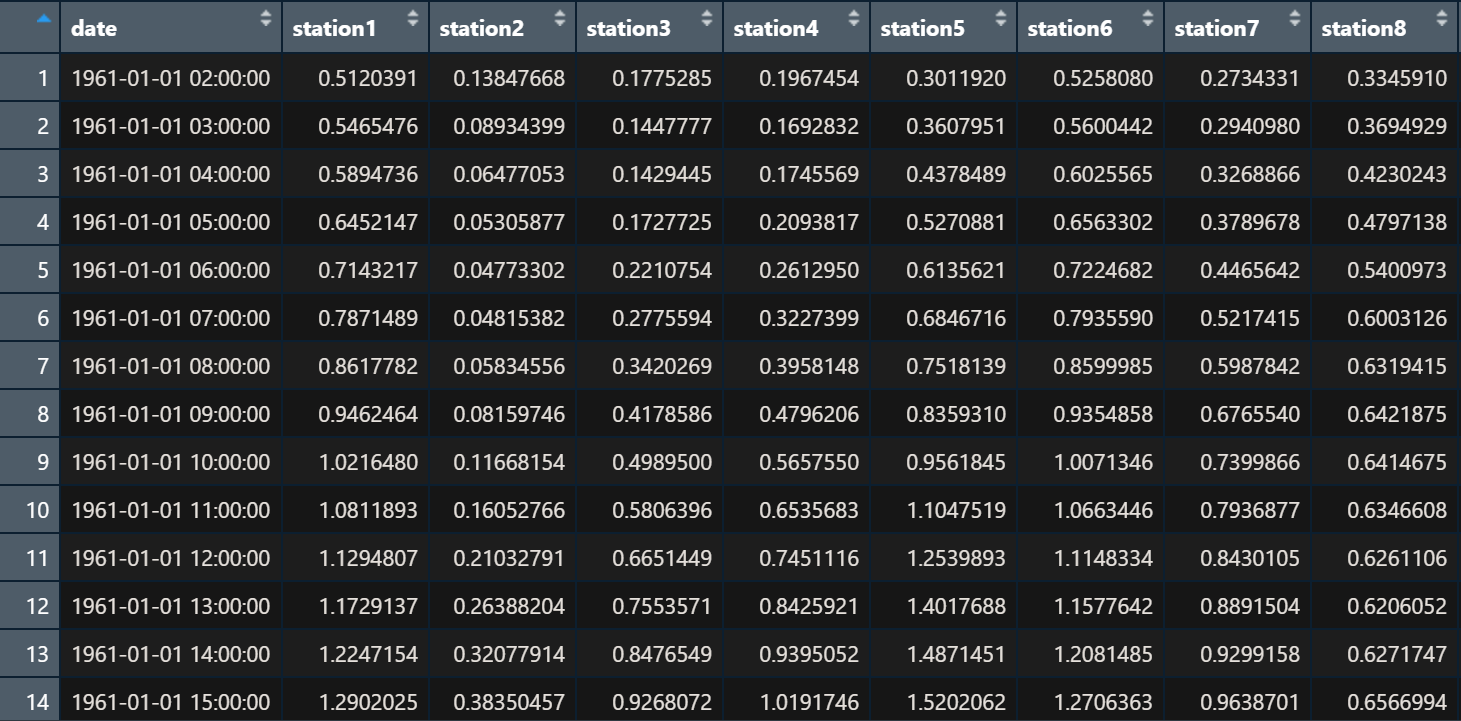
\includegraphics[scale=0.45]{images/data1.png}
	\caption{Extrait du dataframe \textit{DonneesVagues}}
	\label{data1}
\end{figure}

\begin{figure}[htp] 
	\centering
	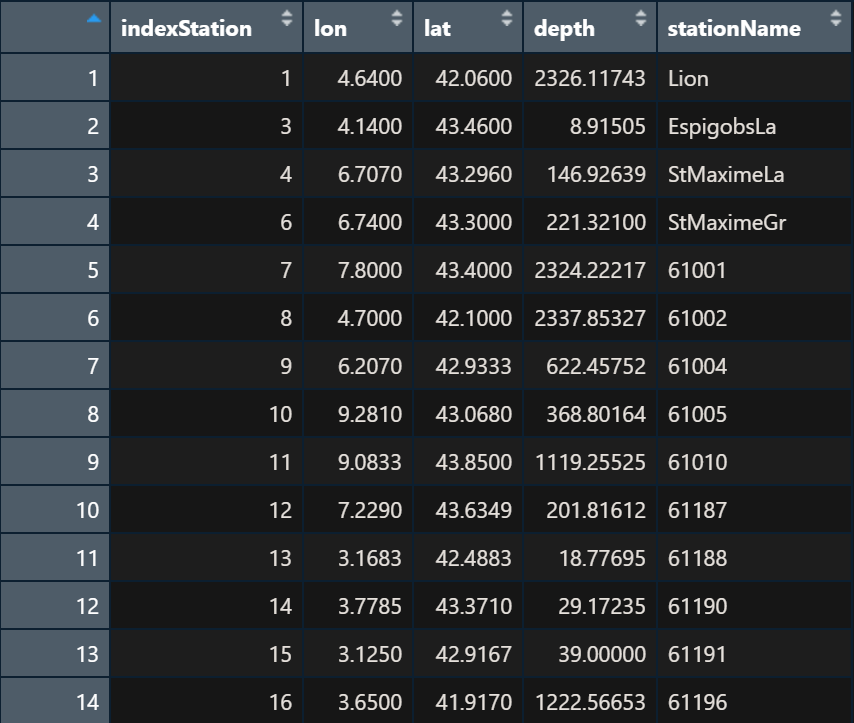
\includegraphics[scale=0.45]{images/data2.png}
	\caption{Extrait du dataframe \textit{DonneesStations}}
	\label{data2}
\end{figure}

\begin{figure}[htp] 
	\centering
	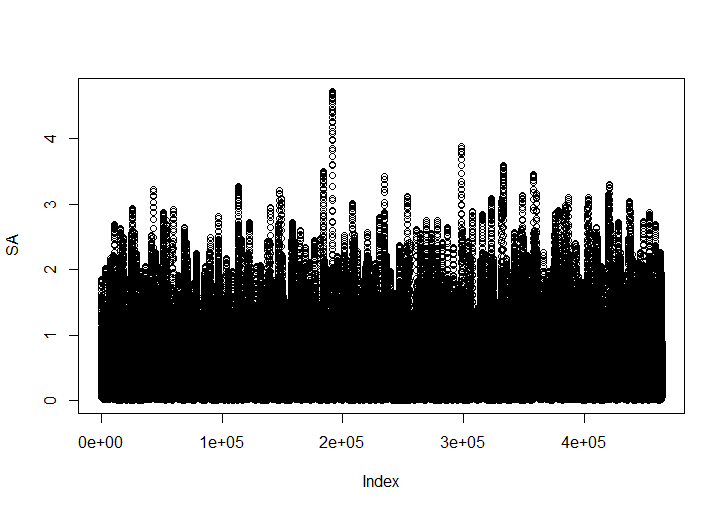
\includegraphics[scale=0.45]{images/graph_data.png}
	\caption{Nuage de points des données \textit{DonneesVagues}}
	\label{data}
\end{figure}

\newpage

Dans ce projet nous réaliserons dans un premier temps les analyses dans le cas univarié, c'est à dire en ne considérant qu'une seule station puis nous ferons une analyse bivariée en considérant cette fois-ci plusieurs stations.

\section{Partie Univariée}
Dans cette partie nous serons dans le cas univarié et nous considérerons la station 2.
Pour mener à bien les analyses nous mettrons en œuvre deux approches. Dans un premier temps nous utiliserons la méthode \textit{GEV} (Generalized Extreme Value) puis dans un second temps nous utiliserons la méthode \textit{GPD}(Generalized Pareto
distribution).
\subsection{Approche GEV}
Pour réaliser l'étude avec l'approche GEV nous allons nous aider de la méthode par blocs.

Au départ, on suppose avoir des réalisations indépendantes et de même loi F d’un certain
phénomène d’intérêt : $X_1, X_2,\dots, X_k$. \\
Dans notre cas nous avons la station 2 comme station de référence (SA).
Pour obtenir un échantillon de max, on découpe les données en m blocs de
même taille n:
\[
	\underbrace{X_1, X_2,\dots, X_n}_{Z1}| \underbrace{X_{n+1}, X_{n+2},\dots, X_{2n}}_{Z2}| \dots |\underbrace {X_{(m-1)n+1}, \dots, X_{mn}}_{Zm}|
\]

On obtient alors un échantillon de $m$ réalisations de loi GEV : $Z_1, Z_2,\dots, Z_m$.

 Afin de faire des analyses de bonnes qualités il est nécessaire de sélectionner une taille de bloc $n$ adéquat. comme il a été dit précédemment, le dataframe \textit{DonneesVagues} est composé de $464280$ lignes.
Afin de choisir une bonne valeur de $n$, nous avons fait un script (disponible en annexe) qui affiche tous les diviseurs de $464280$, ces derniers sont affichés en figure \ref{diviseurs}. À partir de là nous avons pu tester plusieurs valeurs de $m$ et nous avons finalement pris $m=2980$. Nous aurons donc $2980$ blocs tous de même taille $n=159$. Nous allons maintenant justifier pourquoi nous avons décidé de retenir cette valeur. \\
Les points du graphique de la figure \ref{graph_max}, correspondent aux maximums de chaque bloc. Comme on peut le voir, le nuage de points obtenu est assez dispersé ce qui nous conforte dans l'idée que le paramètre $n$ a été bien choisi. \\
D'autre part, nous allons également nous appuyer sur le graphique du \textit{Quantile plot} afin de voir si le paramètre $n$ a bien été choisi. On rappelle que le Quantile plot est le nuage de points: \\

\[
	\Bigl\{\Big(\widehat{G}^{-1}\Big(\frac{i}{m+1}\Big),z_{i,m}\Big), i = 1,\dots, m\Bigr\}
\]

Où

\[
	\widehat{G}(\frac{i}{m+1}) = \widehat{\mu} - \frac{\widehat{\sigma}}{\widehat{\gamma}} \Big[ 1- \Big(-log\Big(\frac{i}{i+1}\Big)\Big)^{-\widehat{\gamma}}\Big]
\]

Si l'on observe le graphique de la figure \ref{qplot}, on s'aperçoit que les points du nuage sont proches de la diagonale (ligne bleue) donc l'ajustement est de bonne qualité, la taille des blocs retenue pour l'approche GEV a donc été bien choisie. 


\begin{figure}[htp] 
	\centering
	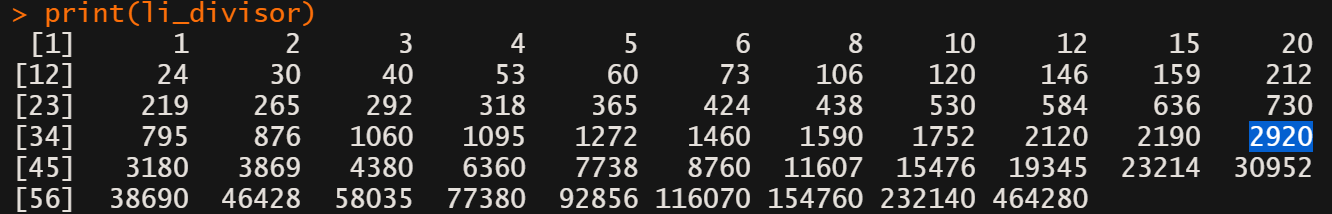
\includegraphics[scale=0.45]{images/diviseurs.png}
	\caption{liste des diviseurs de $464280$}
	\label{diviseurs}
\end{figure}
 
 \begin{figure}[htp] 
 	\centering
 	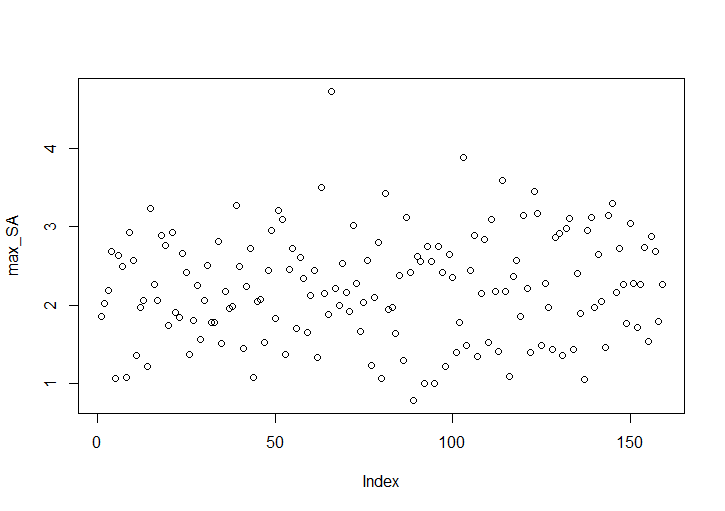
\includegraphics[scale=0.45]{images/graph_max.png}
 	\caption{nuage de points obtenu avec la méthode par bloc}
 	\label{graph_max}
 \end{figure}

\begin{figure}[htp] 
	\centering
	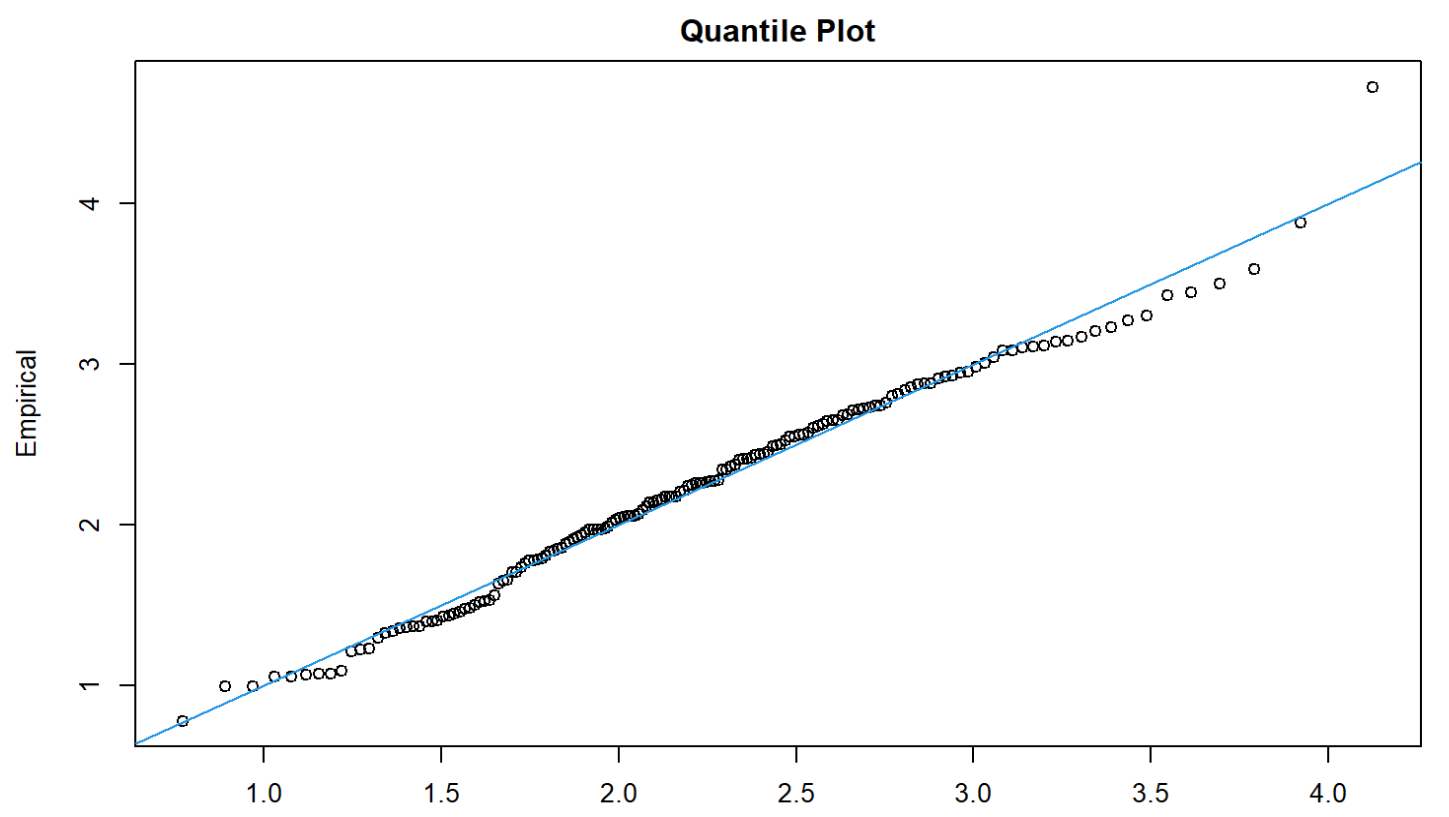
\includegraphics[scale=0.45]{images/quantilePlotUnivarie.png}
	\caption{Quantile plot}
	\label{qplot}
\end{figure}

\newpage

\subsubsection{Niveaux de retour associés aux périodes de retour $100$, $500$ et $1000$}

Dans cette sous-section, nous allons nous intéresser aux niveaux de retour $x_{\frac{1}{T}}$ associés aux périodes de retour $T = \frac{1}{q}$ pour $T \in \{100,500,1000\}$. L'on souhaite connaître le niveau qui sera dépassé tous les $100$, $500$ et $1000$ ans.

\begin{table}[htp]
	\center
	\begin{tabular}{|c||c|c|c|}
		\hline
		\diagbox{Niveau de retour}{Périodes ou Années $T$} & $T = 100$ & $T = 500$ & $T = 1000$\\
		\hline
		$x_{\frac{1}{T}}$ & $3.99003$ & $4.413046$ & $4.563588$ \\
		\hline
	\end{tabular}
	\caption{Niveaux de retour associés aux périodes de retour $T$}
	\label{tab1}
\end{table}

\begin{table}[htp]
	\center
	\begin{tabular}{|c||c|c|c|}
		\hline
		\diagbox{Intervalles de confiance}{Périodes ou Années $T$} & $T = 100$ & $T = 500$ & $T = 1000$\\
		\hline
		IC de niveau $1-\alpha = 95\%$ & $[3.691942,4.288119]$ & $[3.974492,4.851601]$ & $[4.059768, 5.067409]$ \\
		\hline
	\end{tabular}
	\caption{Intervalles de confiance des niveaux de retour $x_{\frac{1}{T}}$}
	\label{tab2}
\end{table}
En regardant les valeurs des niveaux de retour affichées dans le tableau \ref{tab1}, on constate qu'elles sont bien toutes comprises dans leurs intervalles de confiance respectifs (voir tableau \ref{tab2}). Cela nous confirme une fois de plus que la taille $n$ des blocs choisis pour l'approche GEV est bonne. \\
D'autre part, on remarque que plus la période de retour $T$ est grande et plus le niveau de retour augmente. Cette augmentation des hauteurs de vagues peut s'expliquer par la montée du niveau de la mer au fil des années. On pourrait donc se demander si des plages comme celles de Carnon, Palavas ou encore La Grande-Motte existeront toujours dans 1000 ans ?

\subsection{Approche GPD}
Pour mener cette fois-ci l'étude avec l'approche GPD, il faut déterminer la valeur du seuil à utiliser. Une fois de plus, si l'on souhaite réaliser de bonnes analyses, il faut être vigilant au seuil que l'on choisit. Afin de déterminer ce dernier, nous allons nous aider de la figure \ref{mean_res}, sur laquelle est tracé le diagramme de durée de vie résiduelle moyenne (Mean residual life plot).

\begin{figure}[htp] 
	\centering
	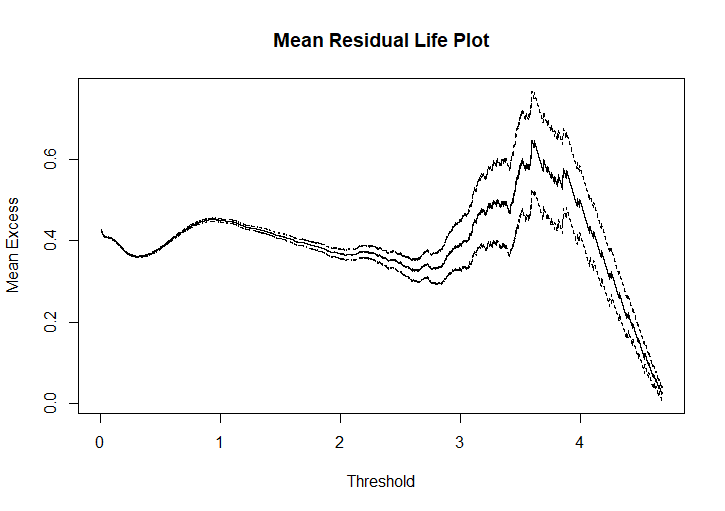
\includegraphics[scale=0.45]{images/res_mean.png}
	\caption{diagramme de durée de vie résiduelle moyenne}
	\label{mean_res}
\end{figure}
Sur la figure \ref{mean_res}, on voit que les pics significatifs sont atteints pour des valeurs de seuil (Threshold) valant approximativement $2.7$ et $3.65$. Nous avons donc testé ces deux valeurs de seuil et nous avons finalement retenu la valeur $3.65$. Nous allons maintenant justifier pourquoi nous avons décidé de retenir cette dernière valeur.

\begin{figure}[htp] 
	\centering
	\subfloat[seuil $\approx 2.7$]{%
		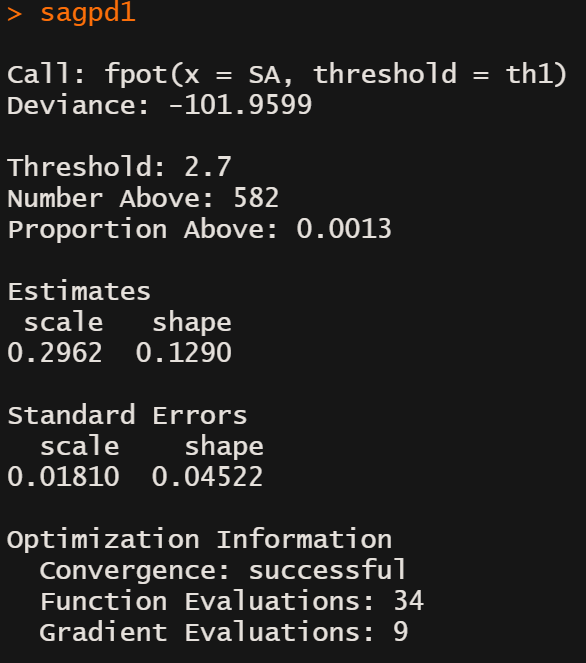
\includegraphics[scale=0.4]{images/sumBadth.png}%
	}%
	\hfill%
	\subfloat[seuil $\approx 3.65$]{%
		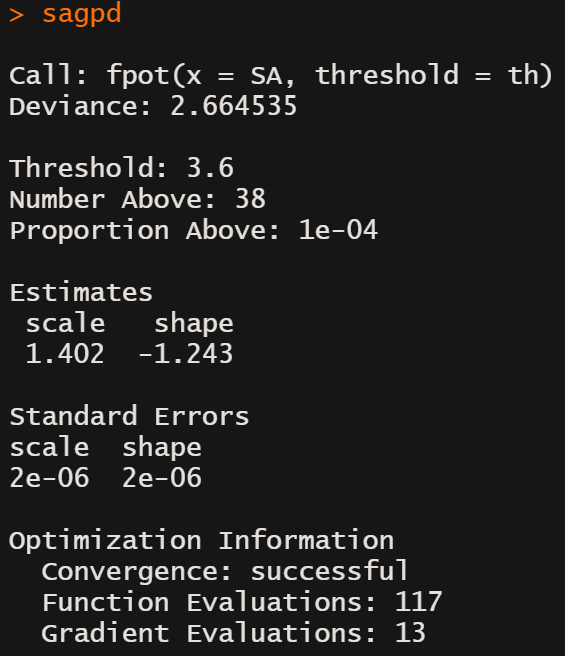
\includegraphics[scale=0.4]{images/sumGoodth.png}%
	}%
	\caption{Résultats donnés en sortie de la fonction \textit{fpot} pour les 2 seuils}
	\label{summary}
\end{figure}

\begin{figure}[htp] 
	\centering
	\subfloat[seuil $\approx 2.7$]{%
				\includegraphics[scale=0.4]{images/qPlotBadth.png}%
			}%
	\hfill%
	\subfloat[seuil $\approx 3.65$]{%
				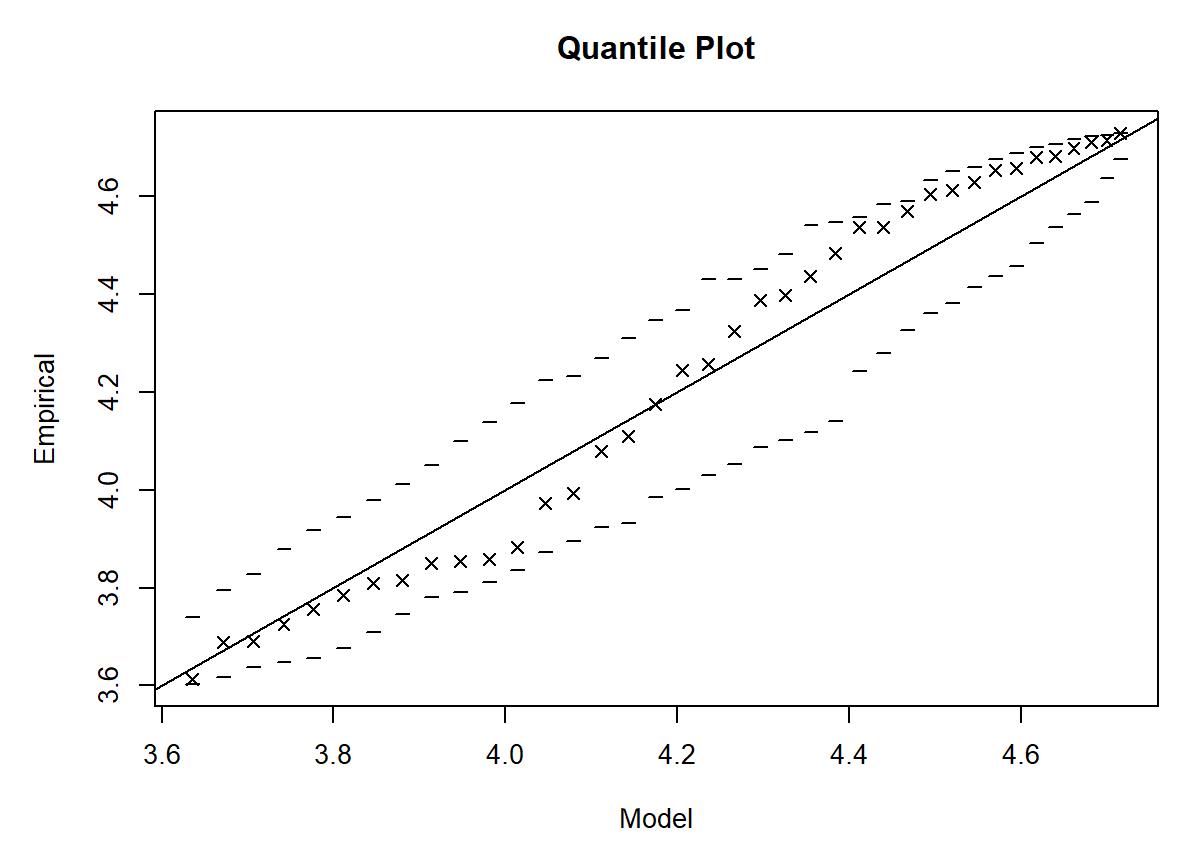
\includegraphics[scale=0.4]{images/qPlotGoodth.png}%
			}%
	\caption{Quantile plot des 2 seuils}
	\label{graph}
\end{figure}

En observant les résultats affichés sur les captures d'écran de la figure \ref{summary}, on voit que la proportion de valeurs dépassant le seuil (proportion above) est plus faible dans le cas où ce dernier vaut $\approx 3.65$ que dans le cas où il vaut $\approx 2.7$. \\
De plus, en observant les graphiques (\textit{Quantile plot}) de la figure \ref{graph}, on remarque que le nuage de points du seuil $\approx 3.65$ est plus proche de la droite en diagonale que le nuage de points du seuil $\approx 2.7$. \\
Ces résultats nous ont donc poussés à choisir le seuil$=3.65$ car il nous permettra de faire une analyse de meilleure qualité qu'avec l'autre valeur de seuil.

\subsubsection{Niveaux de retour associés aux périodes de retour $100$, $500$ et $1000$}
Maintenant que nous avons déterminer le seuil (threshold), nous allons nous intéresser comme dans le cas de l'approche GEV, aux niveaux de retour $x_{\frac{1}{T}}$ associés aux périodes de retour $T = \frac{1}{q}$ pour $T \in \{100,500,1000\}$. L'on souhaite connaître le niveau qui sera dépassé tous les $100$, $500$ et $1000$ ans avec l'approche GPD.

\begin{table}[htp]
	\center
	\begin{tabular}{|c||c|c|c|}
		\hline
		\diagbox{Niveau de retour}{Périodes ou Années $T$} & $T = 100$ & $T = 500$ & $T = 1000$\\
		\hline
		$x_{\frac{1}{T}}$ & $4.686475$ & $4.72502$ & $4.723653$ \\
		\hline
	\end{tabular}
	\caption{Niveaux de retour associés aux périodes de retour $T$}
	\label{tab3}
\end{table}
Quand on regarde le tableau \ref{tab3}, on constate que le niveau de retour pour la période $T=500$ est supérieur à celui pour la période $T=100$. Cependant, pour la période $T=1000$, la valeur de $x_{\frac{1}{T}}$ est inférieur à celle trouvée pour $T = 500$. Ce qui est différent des résultats obtenus avec l'approche GEV. En effet, pour rappel, avec l'approche GEV on avait trouvé que plus la période de retour $T$ était grande et plus le niveau de retour augmentait, ce qui était cohérent avec la montée des eaux. Dans le cas de ces données, l'approche GEV est donc peut être préférable car elle fournit des résultats plus cohérents que ceux obtenus avec l'approche GPD.

\section{Partie bivariée}
Dans cette nouvelle partie, on se place maintenant dans le cas bivarié.
L'objectif sera de prédire la valeur du quantile extrême $z_p$ vérifiant:
\begin{equation}
	\label{quantile_extreme}
	\mathbb{P}(X > z_p | Y > y) = \frac{\mathbb{P}(X > z_p \cap Y > y)}{\mathbb{P}(Y > y)}
\end{equation}
avec $p$ petit et où $Y$ correspond à la hauteur de vagues associées à la station 2 ($S_A$) et $X$ à la hauteur de vagues associées à la station 9 ($S_B$). \\
Pour mener à bien les analyses dans toute la suite de ce projet, nous mettrons en œuvre uniquement l'approche \textit{GEV} (Generalized Extreme Value) car nous avons vu précédemment que cette dernière fournissait de meilleurs résultats que l'approche GPD dans le cas de nos données. Tout comme dans le cas univarié, nous allons nous aider de la méthode par blocs. Afin de réaliser des analyses de bonnes qualités, nous devons correctement choisir la taille $n$ des blocs. En nous aidant encore une fois du script (disponible en annexe) affichant tous les diviseurs de $464280$, on décide de prendre $m = 2980$ blocs, tous de même taille $n = 159$.

\subsection{Analyse entre les stations 2 et 9}

Sur la figure \ref{max_SB_SA} nous avons tracé deux nuages de points. Les points du nuage rouge correspondent aux maximums de chaque bloc dans le cas de la station $S_B$ et ceux du nuage bleu aux maximums de chaque bloc dans le cas de la station $S_A$. Les points des deux nuages sont assez bien dispersés.
\begin{figure}[htp] 
	\centering
	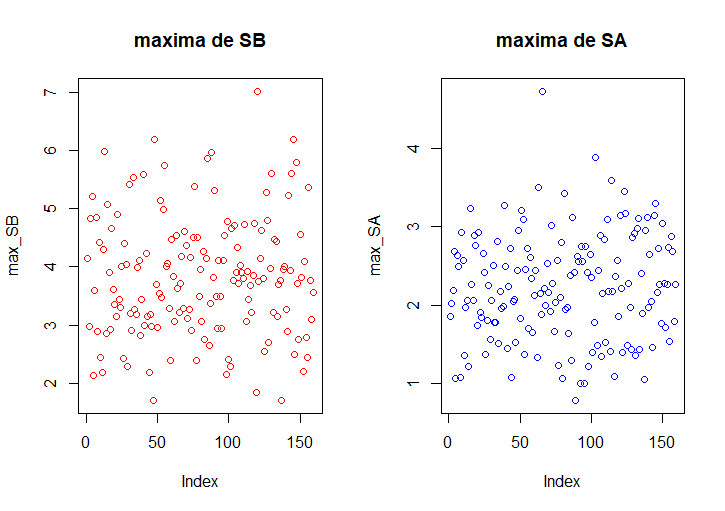
\includegraphics[scale=0.45]{images/max_SB_SA.png}
	\caption{Nuage de points obtenu avec la methode par bloc pour $S_B$ et $S_A$}
	\label{max_SB_SA}
\end{figure}

Nous allons maintenant effectuer un ajustement par une loi GEV sur chacune de deux marginales et nous allons récupérer les paramètres pour chaque ajustement des marginales. Nous les avons affichés dans le tableau \ref{param}.

\begin{table}[htp]
	\center
	\begin{tabular}{|c||c|c|}
		\hline
		 & Paramètres $S_A$ & Paramètres $S_B$\\
		\hline
		$\widehat{\mu}$ & $1.9483809$ & $3.4137728$ \\
		\hline
		$\widehat{\sigma}$ & $0.6317954$ & $0.9391569$ \\
		\hline
		$\widehat{\gamma}$ & $-0.1636501$ & $-0.1620597$ \\
		\hline
	\end{tabular}
	\caption{paramètres des ajustement des marginales}
	\label{param}
\end{table}

Calculons la probabilité de l'équation \ref{quantile_extreme}. \\
Les paramètres du tableau \ref{param} vont nous aider à calculer cette probabilité. En effet, ils seront utilisés dans la fonction $pgev$ de $R$ qui va nous permettre de déterminer le dénominateur $\mathbb{P}(Y > y)$.\\
on rappelle qu'ici, à titre d'exemple nous avons choisi la valeur $y = 4$. \\
Après calcul, on trouve que $\mathbb{P}(Y > 4)=0.4041958$. \\
Nous avons également besoin de calculer le numérateur à savoir $\mathbb{P}(X > z_p \cap Y > y)$. \\
La fonction $fbvevd$ de $R$ nous permettra de récupérer les paramètres ($loc$,$scale$ et $shape$) nécessaires au calcul du numérateur. La valeur de ce dernier est ensuite obtenue via la fonction $pbvevd$ et on obtient que $\mathbb{P}(X > z_p \cap Y > 4) = 0.01589988$.\\
On en déduit donc que $\mathbb{P}(X > z_p | Y > 4) = 0.03933707$. C'est à dire que la probabilité que la hauteur de la vague de la station 9 soit supérieure $z_p$ sachant que la hauteur de la vague de la station 2 est supérieure à 4 vaut environ $3.93\%$.

\vspace{4mm}

Nous allons maintenant procéder à une analyse bivariée entre les stations 2 et 9. La figure \ref{double_max} représente les hauteurs maximales des vagues selon les blocs pour les stations 2 et 9. Après observation de ce nuage de points, il semblerait que les données des deux stations ne soient pas corrélées entre elles car le nuage est assez dispersé. 

\begin{figure}[htp] 
	\centering
	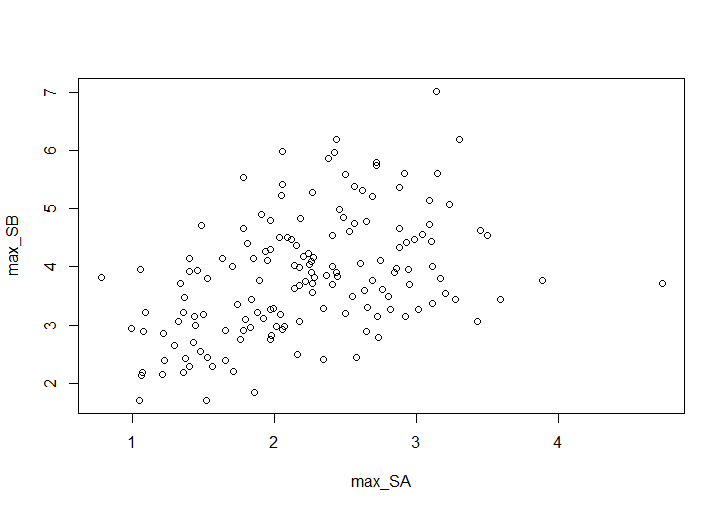
\includegraphics[scale=0.45]{images/double_max.png}
	\caption{hauteurs maximales des vagues selon les blocs pour les station 2 et 9}
	\label{double_max}
\end{figure}

Dans la suite de cette partie, nous allons faire des analyses plus fines afin de vérifier si notre hypothèse d'indépendance entre les données des deux stations est juste ou pas. Pour ce faire nous allons utiliser deux différents modèles d'estimation paramétrique à savoir le modèle logistique et celui logistique asymétrique. Nous allons ensuite sélectionner le meilleur de ces deux modèles à l'aide du critère AIC.
D'après la source \cite{AIC}, le critère AIC se définit de la manière suivante:
\[
	AIC = 2k - 2 ln(L)
\]

Où $k$ est le nombre de paramètres à estimer du modèle et $L$ est le maximum de la fonction de vraisemblance du modèle. \\
D'après la capture d'écran de la figure \ref{AIC_2_9}, le modèle logistique est celui ayant l'AIC le plus faible avec une valeur de $763.3703$ contre $766.2632$ pour le modèle logistique asymétrique. On en déduit donc que le meilleur des deux modèles est celui logistique ($log$) et c'est donc ce dernier que nous sélectionnerons.

\begin{figure}[htp] 
	\centering
	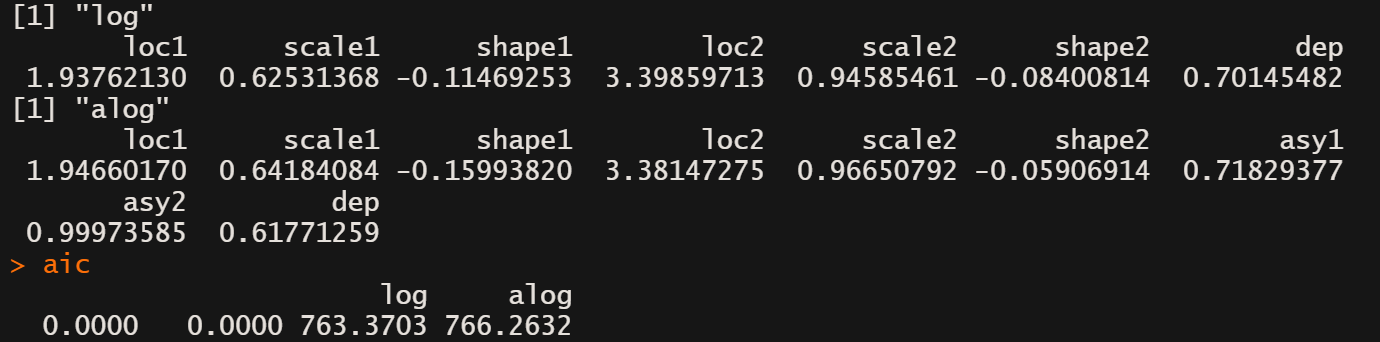
\includegraphics[scale=0.45]{images/AIC_stations2_9.png}
	\caption{AIC des modèles $log$ et $alog$}
	\label{AIC_2_9}
\end{figure}

Ajustons maintenant le modèle $log$. En observant la figure \ref{dependance_log}, on voit que la valeur du paramètre dépendance vaut $0.3738562$. Il est proche de zéro, on en déduit donc que les données des stations 9 et 2 ne sont pas corrélées entre elles. Notre hypothèse d'indépendance des données est donc valide.

\begin{figure}[htp] 
	\centering
	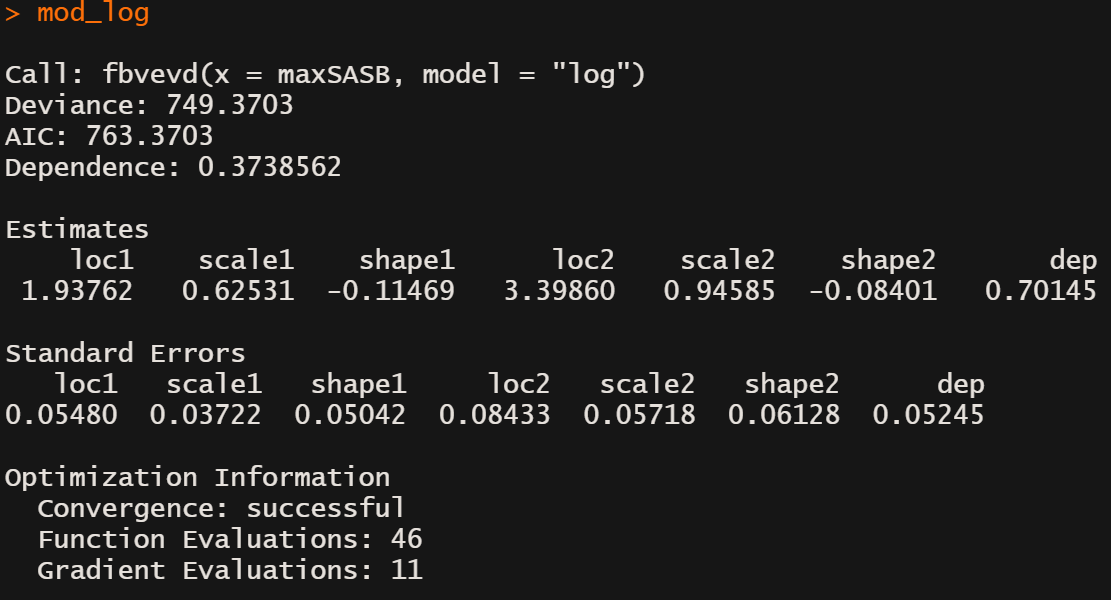
\includegraphics[scale=0.45]{images/dependance_log.png}
	\caption{Vérification de la validité de l'hypothèse d'indépendance}
	\label{dependance_log}
\end{figure}

\subsection{Analyse entre les stations 2 et 7}
Dans cette partie, nous cherchons dans un premier temps une station notée $S_C$ qui est plus proche de $S_A$ que $S_B$. Une fois que nous l'aurons trouvée, nous ferons une analyse entre notre station de référence $S_A$ et la nouvelle station $S_C$.
Pour déterminer $S_C$, nous avons utilisé la norme euclidienne présentée dans le document \cite{norme_euclid} et nous avons appliqué les formules \ref{euclidienne1} et \ref{euclidienne2} sur les coordonnées géographiques des stations (longitude et latitude) disponibles dans le dataframe \textit{DonneesStations}.

\begin{equation}
	\label{euclidienne1}
	\sqrt \Big(  (longitude[S_A] - longitude[S_C])^2 + (latitude[S_A] - latitude[S_C])^2 \Big)
\end{equation}

\begin{equation}
	\label{euclidienne2}
	\sqrt \Big(  (longitude[S_C] - longitude[S_B])^2 + (latitude[S_C] - latitude[S_B])^2 \Big)
\end{equation}

En prenant $S_C = station7$, nous obtenons après application des formules \ref{euclidienne1} et \ref{euclidienne2} que :
\begin{align*}
	|| \overrightarrow{S_A S_C} || &=  2.13305 \\
	|| \overrightarrow{S_C S_B} || &=  3.018848
\end{align*}
Donc le choix de la station 7 est valide car cette dernière est effectivement plus proche de $S_A$ que $S_B$.

\vspace{3mm}

Sur la figure \ref{max_SA_SC} nous avons tracé deux nuages de points. Les points du nuage magenta correspondent aux maximums de chaque bloc dans le cas de la station $S_C$ et ceux du nuage bleu clair aux maximums de chaque bloc dans le cas de la station $S_A$. Les points des deux nuages sont assez bien dispersés.
\begin{figure}[htp] 
	\centering
	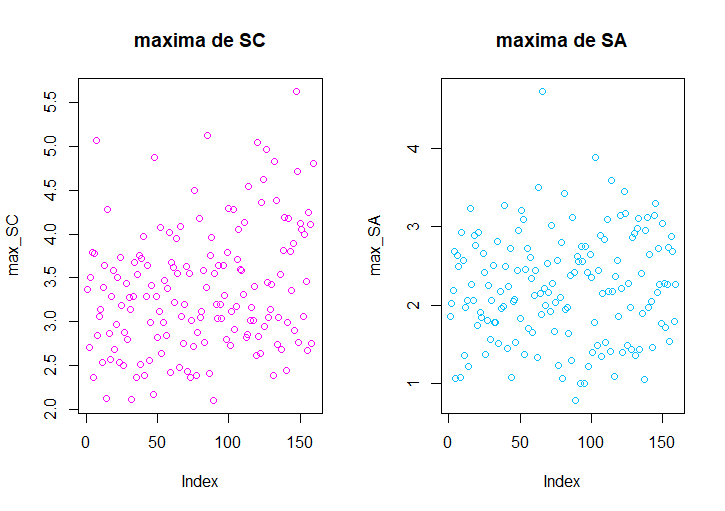
\includegraphics[scale=0.45]{images/max_SA_SC.png}
	\caption{Nuage de points obtenu avec la méthode par bloc pour $S_A$ et $S_C$}
	\label{max_SA_SC}
\end{figure}

Nous allons maintenant procéder à une analyse bivariée entre les stations 2 et 7. La figure \ref{double_max2} représente les hauteurs maximales des vagues selon les blocs pour les stations 2 et 7. Après observation de ce nuage de points, il semblerait que les données des deux stations soient moins dispersées que celles des stations 2 et 9 (voir figure \ref{double_max}).

\begin{figure}[htp] 
	\centering
	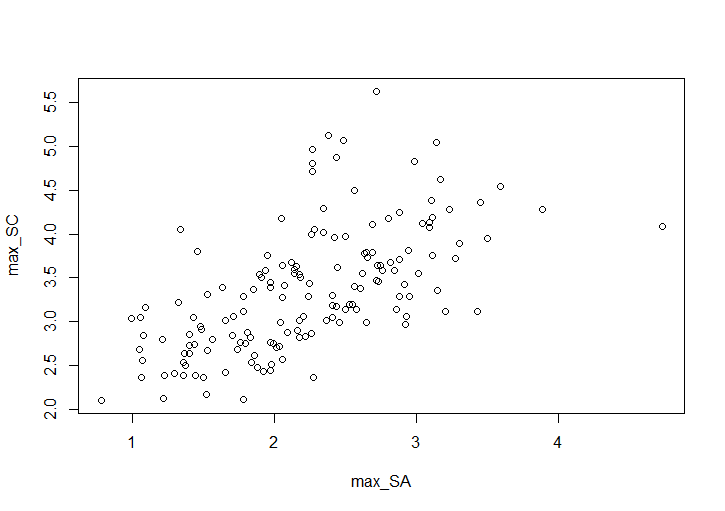
\includegraphics[scale=0.45]{images/double_max2.png}
	\caption{hauteurs maximales des vagues selon les blocs pour les station 2 et 7}
	\label{double_max2}
\end{figure}

Dans la suite de cette partie, nous allons faire des analyses plus fines afin de voir s'il y a plus de corrélations entre les données des stations 2 et 7. Logiquement vu que les stations 2 et 7 sont plus proches l'une de l'autre que les stations 2 et 9, il devrait y avoir ici plus de corrélations. Vérifions le. Pour ce faire nous allons encore une fois utiliser les modèles d'estimation paramétrique logistique et celui logistique asymétrique. Nous allons ensuite sélectionner le meilleur de ces deux modèles à l'aide du critère AIC.

D'après la capture d'écran de la figure \ref{AIC_2_7}, le modèle logistique est celui ayant l'AIC le plus faible avec une valeur de $590.3655$ contre $596.5881$ pour le modèle logistique asymétrique. On en déduit donc que le meilleur des deux modèles est celui logistique ($log$) et c'est donc ce dernier que nous sélectionnerons.

\begin{figure}[htp] 
	\centering
	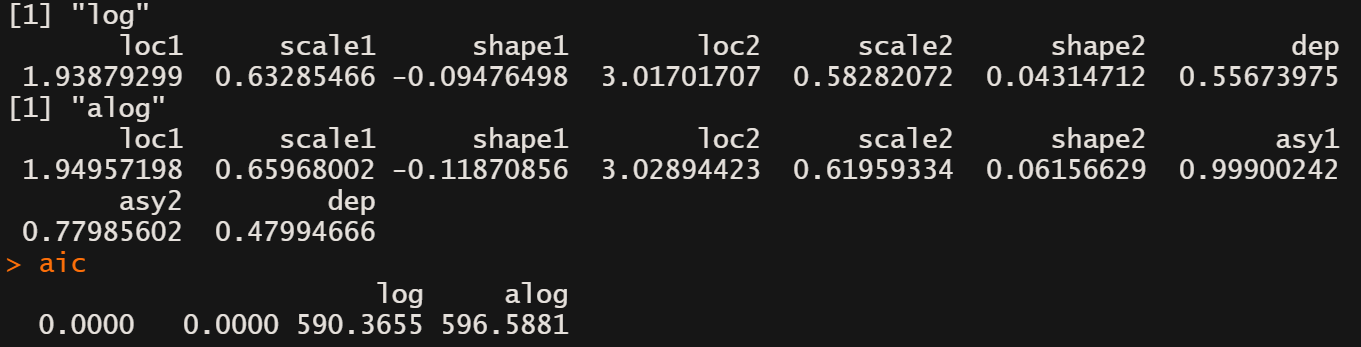
\includegraphics[scale=0.45]{images/AIC_stations2_7.png}
	\caption{AIC des modèles $log$ et $alog$}
	\label{AIC_2_7}
\end{figure}

Ajustons maintenant le modèle $log$. En observant la figure \ref{dependance_log2}, on voit que la valeur du paramètre dépendance vaut $0.5290586$. Il est donc plus grand que dans le cas des stations 2 et 9 (voir figure \ref{dependance_log}). Ceci est parfaitement cohérent avec ce que l'on avait dit précédemment. En effet, plus l'on va prendre des stations proches entre elles et plus il y aura de corrélations entre les données de ces dernières.

\begin{figure}[htp] 
	\centering
	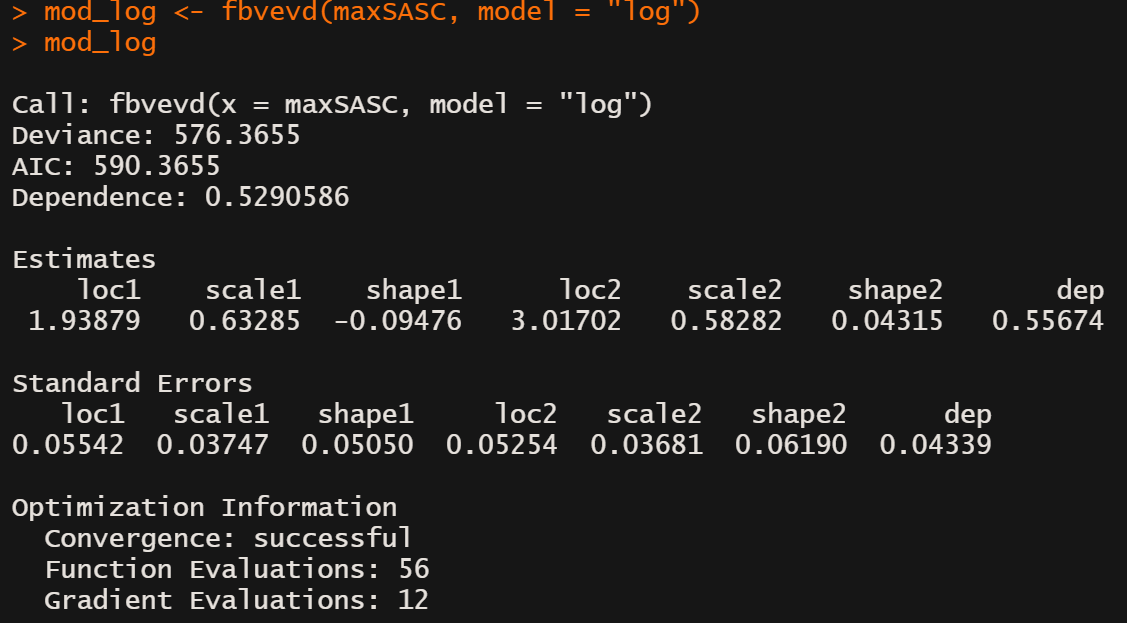
\includegraphics[scale=0.45]{images/dependance_log2.png}
	\caption{Vérification de la validité de l'hypothèse d'indépendance}
	\label{dependance_log2}
\end{figure}


\subsection{Analyse entre les stations 9 et 4}
Dans cette partie, nous cherchons dans un premier temps une station notée $S_D$ qui est plus proche de $S_B$ que $S_A$. Une fois que nous l'aurons trouvée, nous ferons une analyse entre la station $S_B$ et la nouvelle station $S_D$.
Pour déterminer $S_D$, nous avons utiliser comme dans la partie précédente, la norme euclidienne et nous avons appliqué les formules \ref{euclidienne3} et \ref{euclidienne4} sur les coordonnées géographiques des stations (longitude et latitude) disponibles dans le dataframe \textit{DonneesStations}.

\begin{equation}
	\label{euclidienne3}
	\sqrt \Big(  (longitude[S_D] - longitude[S_B])^2 + (latitude[S_D] - latitude[S_B])^2 \Big)
\end{equation}

\begin{equation}
	\label{euclidienne4}
	\sqrt \Big(  (longitude[S_A] - longitude[S_D])^2 + (latitude[S_A] - latitude[S_D])^2 \Big)
\end{equation}

En prenant $S_D = station4$, nous obtenons après application des formules \ref{euclidienne1} et \ref{euclidienne2} que :
\begin{align*}
	|| \overrightarrow{S_B S_D} || &=  2.40698 \\
	|| \overrightarrow{S_A S_D} || &=  2.604918
\end{align*}
Donc le choix de la station 4 est valide car cette dernière est effectivement plus proche de $S_B$ que $S_A$.

\vspace{3mm}

Sur la figure \ref{max_SB_SD} nous avons tracé deux nuages de points. Les points du nuage orange correspondent aux maximums de chaque bloc dans le cas de la station $S_C$ et ceux du nuage vert aux maximums de chaque bloc dans le cas de la station $S_A$. Les points des deux nuages sont assez bien dispersés.
\begin{figure}[htp] 
	\centering
	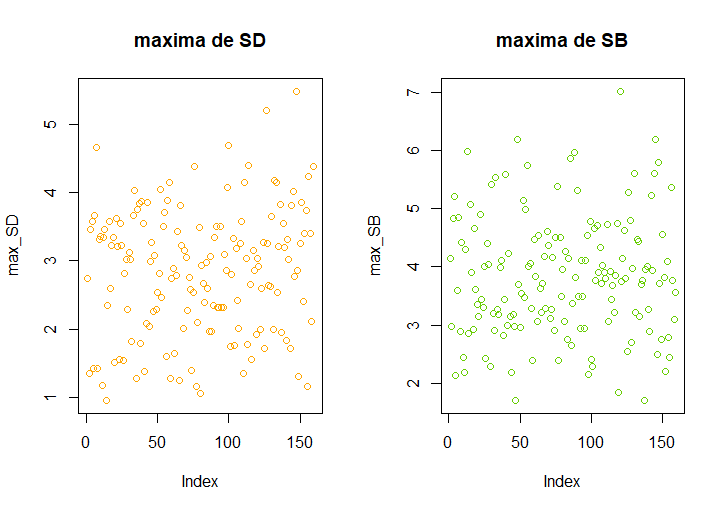
\includegraphics[scale=0.45]{images/max_SB_SD.png}
	\caption{Nuage de points obtenu avec la méthode par bloc pour $S_B$ et $S_D$}
	\label{max_SB_SD}
\end{figure}

Nous allons maintenant procéder à une analyse bivariée entre les stations 9 et 4. La figure \ref{double_max3} représente les hauteurs maximales des vagues selon les blocs pour les stations 9 et 4. Après observation de ce nuage de points, il semblerait que les données des deux stations soient moins dispersées que celles des stations 2 et 9 (voir figure \ref{double_max}).

\begin{figure}[htp] 
	\centering
	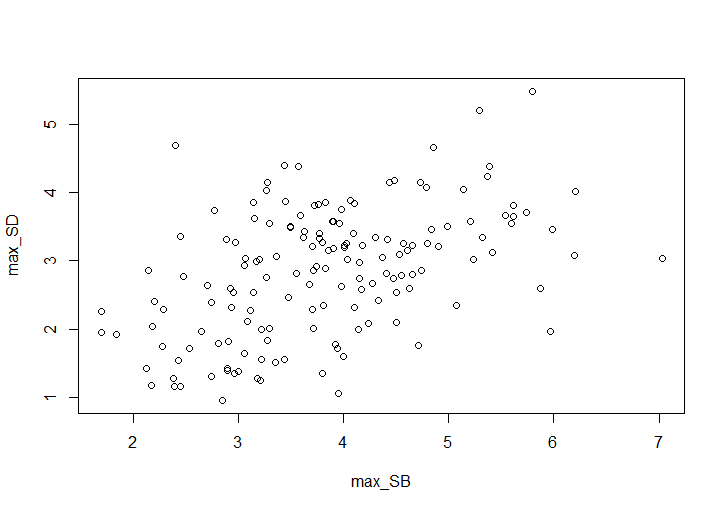
\includegraphics[scale=0.45]{images/double_max3.png}
	\caption{hauteurs maximales des vagues selon les blocs pour les station 9 et 4}
	\label{double_max3}
\end{figure}

Dans la suite de cette partie, nous allons faire des analyses plus fines afin de voir s'il y a plus de corrélations entre les données des stations 9 et 4. Logiquement vu que les stations 9 et 4 sont plus proches l'une de l'autre que les stations 2 et 9, il devrait y avoir ici plus de corrélations. Vérifions le. Pour ce faire nous allons encore une fois utiliser les modèles d'estimation paramétrique logistique et celui logistique asymétrique. Nous allons ensuite sélectionner le meilleur de ces deux modèles à l'aide du critère AIC.

\newpage

D'après la capture d'écran de la figure \ref{AIC_9_4}, le modèle logistique est celui ayant l'AIC le plus faible avec une valeur de $857.6410$ contre $862.1909$ pour le modèle logistique asymétrique. On en déduit donc que le meilleur des deux modèles est celui logistique ($log$) et c'est donc ce dernier que nous sélectionnerons.

\begin{figure}[htp] 
	\centering
	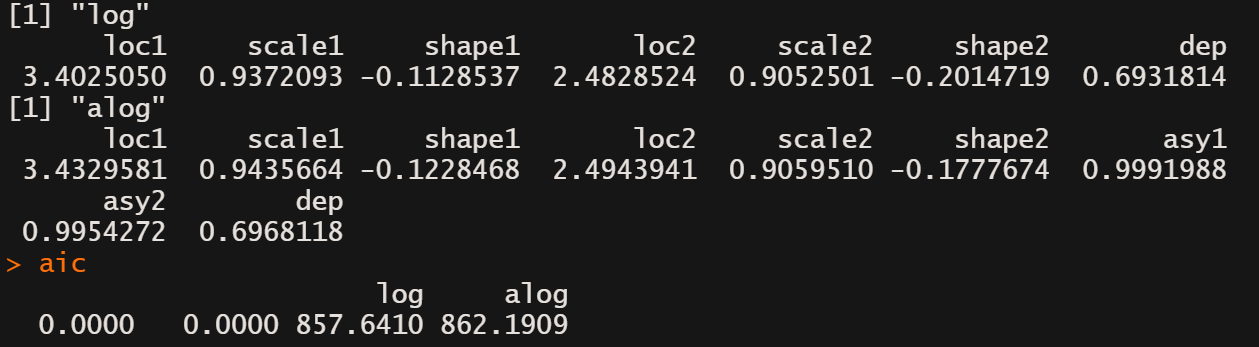
\includegraphics[scale=0.45]{images/AIC_stations9_4.png}
	\caption{AIC des modèles $log$ et $alog$}
	\label{AIC_9_4}
\end{figure}

Ajustons maintenant le modèle $log$. En observant la figure \ref{dependance_log3}, on voit que la valeur du paramètre dépendance vaut $0.383155$. Il est donc légèrement plus grand que dans le cas des stations 2 et 9 (voir figure \ref{dependance_log}). Ici la station $S_D$ est légèrement plus proche de $S_B$ qu'elle ne l'est de $S_A$, c'est pourquoi la corrélation entre les données de $S_B$ et $S_D$ n'est que légèrement plus grande que celle entre les données de $S_A$ et $S_B$. Si l'on voulait avoir une corrélation plus élevée, il faudrait choisir une station qui serait à la fois encore plus proche de $S_B$ et encore plus éloignée de $S_A$. Au final, même si ici la différence est moins marquante que pour la station 2 et 7, on constate toujours que plus l'on va prendre des stations proches entre elles et plus il y aura de corrélations entre les données de ces dernières.

\begin{figure}[htp] 
	\centering
	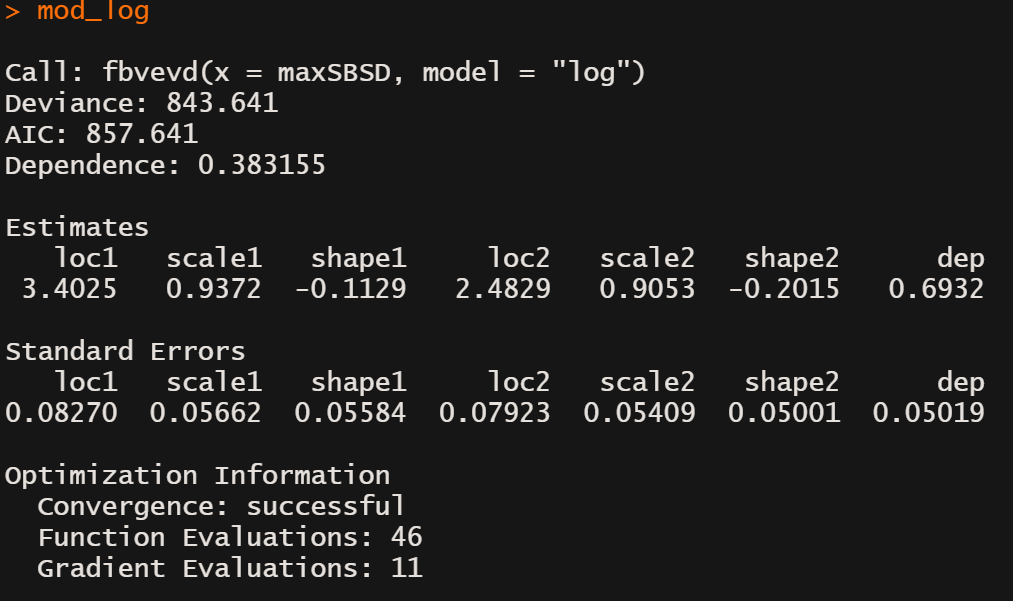
\includegraphics[scale=0.45]{images/dependance_log3.png}
	\caption{Vérification de la validité de l'hypothèse d'indépendance}
	\label{dependance_log3}
\end{figure}

\newpage

\section{Conclusion}
À travers ce projet, nous avons pu voir qu'au fil des années, nous serons confrontés à des valeurs extrêmes de vagues de plus en plus grandes. Cela est sans aucun doute une conséquence de la hausse des températures et en particulier de la montée du niveau des océans. Nous comprenons donc pourquoi la lutte contre le réchauffement climatique est au cœur des enjeux scientifiques actuels. D'autre part, nous avons pu constater que plus nous prendrons des mesures issues de stations proches et plus les données associées à ces dernières seront fortement corrélées. 


\newpage

\section{Annexes}
Ci dessous, l'export de code permettant d'afficher la liste des diviseurs de $464280$.
\lstinputlisting[language=R, firstline=19, lastline=26]{code/script_projet_VE_COME_NIASSE.R}

Dans l'export de code ci dessous on applique la méthode par bloc puis on affiche le nuage de points des maximums des blocs.
\lstinputlisting[language=R, firstline=38, lastline=40]{code/script_projet_VE_COME_NIASSE.R}

La fonction affichée ci-dessous permet d'afficher les graphiques de diagnostics tels que le $Quantile$ $Plot$ et le $Probability$ $Plot$.
\lstinputlisting[language=R, firstline=45, lastline=45]{code/script_projet_VE_COME_NIASSE.R}

Dans l'export de code ci-dessous, on affiche la valeur du niveau de retour $x_{\frac{1}{T}}$ associée à la période de retour $T=100$ ainsi qu'un intervalle de confiance de niveau $1- \alpha = 95\%$
\lstinputlisting[language=R, firstline=49, lastline=59]{code/script_projet_VE_COME_NIASSE.R}

Dans l'export de code ci-dessous, on affiche la valeur du niveau de retour $x_{\frac{1}{T}}$ associée à la période de retour $T=500$ ainsi qu'un intervalle de confiance de niveau $1- \alpha = 95\%$
\lstinputlisting[language=R, firstline=62, lastline=72]{code/script_projet_VE_COME_NIASSE.R}

\newpage

Dans l'export de code ci-dessous, on affiche la valeur du niveau de retour $x_{\frac{1}{T}}$ associée à la période de retour $T=1000$ ainsi qu'un intervalle de confiance de niveau $1- \alpha = 95\%$
\lstinputlisting[language=R, firstline=75, lastline=85]{code/script_projet_VE_COME_NIASSE.R}

La fonction ci-dessous affiche le \textit{Mean Residual Life Plot}
\lstinputlisting[language=R, firstline=88, lastline=88]{code/script_projet_VE_COME_NIASSE.R}

Via l'export de code ci-dessous, on met en œuvre l'approche GPD avec la fonction $fpot$ et on affiche les graphiques de diagnostics (th correspond au seuil threshold).
\lstinputlisting[language=R, firstline=97, lastline=102]{code/script_projet_VE_COME_NIASSE.R}

L'export de code ci-dessous permet de calculer le niveau de retour $x_{\frac{1}{T}}$ associé à la période de retour $T = 100$ avec l'approche GPD, $n = 2920$ correspond au nombre de blocs.
\lstinputlisting[language=R, firstline=107, lastline=111]{code/script_projet_VE_COME_NIASSE.R}

L'export de code ci-dessous permet de calculer le niveau de retour $x_{\frac{1}{T}}$ associé à la période de retour $T = 500$ avec l'approche GPD, $n = 2920$ correspond au nombre de blocs.
\lstinputlisting[language=R, firstline=114, lastline=118]{code/script_projet_VE_COME_NIASSE.R}

L'export de code ci-dessous permet de calculer le niveau de retour $x_{\frac{1}{T}}$ associé à la période de retour $T = 1000$ avec l'approche GPD, $n = 2920$ correspond au nombre de blocs.
\lstinputlisting[language=R, firstline=120, lastline=124]{code/script_projet_VE_COME_NIASSE.R}

\newpage

Ajustement par une loi GEV pour chacune des deux marginales. \\
Récupération des paramètres chaque ajustement des marginales.

\lstinputlisting[language=R, firstline=157, lastline=168]{code/script_projet_VE_COME_NIASSE.R}

Calcul du dénominateur $\mathbb{P}(Y > y)$
\lstinputlisting[language=R, firstline=173, lastline=176]{code/script_projet_VE_COME_NIASSE.R}

Avec la commande ci dessous, on récupère les paramètres utiles pour calculer le numérateur \\ 
$\mathbb{P}(X > z_p \cap Y > y)$ 
\lstinputlisting[language=R, firstline=179, lastline=179]{code/script_projet_VE_COME_NIASSE.R}

Via l'export de code ci-dessous, on calcule le numérateur $\mathbb{P}(X > z_p \cap Y > y)$
\lstinputlisting[language=R, firstline=185, lastline=188]{code/script_projet_VE_COME_NIASSE.R}

Affichage du nuage de points bivarié
\lstinputlisting[language=R, firstline=192, lastline=192]{code/script_projet_VE_COME_NIASSE.R}

L'export de code ci-dessous nous permet de sélectionner le meilleur modèle à l'aide du critère AIC
\lstinputlisting[language=R, firstline=195, lastline=202]{code/script_projet_VE_COME_NIASSE.R}

L'export de code ci-dessous nous permet d'ajuster le meilleur modèle et de vérifier le niveau de corrélation des données
\lstinputlisting[language=R, firstline=208, lastline=211]{code/script_projet_VE_COME_NIASSE.R}

Dans l'export de code ci-dessous, on calcule la distance séparant la station 2 et la station 7 ainsi que la distance séparant la station 9 avec la station 7.
\lstinputlisting[language=R, firstline=225, lastline=226]{code/script_projet_VE_COME_NIASSE.R}

Affichage du nuage de points bivarié pour les stations 2 et 7
\lstinputlisting[language=R, firstline=248, lastline=248]{code/script_projet_VE_COME_NIASSE.R}

L'export de code ci-dessous nous permet de sélectionner le meilleur modèle à l'aide du critère AIC
\lstinputlisting[language=R, firstline=251, lastline=258]{code/script_projet_VE_COME_NIASSE.R}

L'export de code ci-dessous nous permet d'ajuster le meilleur modèle et de vérifier le niveau de corrélation des données
\lstinputlisting[language=R, firstline=264, lastline=267]{code/script_projet_VE_COME_NIASSE.R}

Dans l'export de code ci-dessous, on calcule la distance séparant la station 4 et la station 9 ainsi que la distance séparant la station 4 avec la station 2.
\lstinputlisting[language=R, firstline=272, lastline=273]{code/script_projet_VE_COME_NIASSE.R}

Affichage du nuage de points bivarié pour les stations 4 et 9
\lstinputlisting[language=R, firstline=294, lastline=294]{code/script_projet_VE_COME_NIASSE.R}

L'export de code ci-dessous nous permet de sélectionner le meilleur modèle à l'aide du critère AIC
\lstinputlisting[language=R, firstline=297, lastline=304]{code/script_projet_VE_COME_NIASSE.R}

L'export de code ci-dessous nous permet d'ajuster le meilleur modèle et de vérifier le niveau de corrélation des données
\lstinputlisting[language=R, firstline=310, lastline=313]{code/script_projet_VE_COME_NIASSE.R}

\newpage

\section{Bibliographie}

\renewcommand\refname{}
\begin{thebibliography}{9}
	\bibitem{golfLion}
	\url{https://reporterre.net/Le-golfe-du-Lion-est-tres-vulnerable-a-la-montee-des-eaux}
	page web rédigée par Alexandre Brun et Benoît Devillers
	
	\bibitem{AIC}
	\url{https://fr.wikipedia.org/wiki/Crit%C3%A8re_d%27information_d%27Akaike}
	page web Wikipédia
	
	\bibitem{norme_euclid}
	\url{https://www.normalesup.org/~simonet/teaching/caml-prepa/tp-caml-2001-02.pdf}
	TP MPSI – Option Informatique rédigé par Vincent Simonet en 2021
\end{thebibliography}

\end{document}
